\documentclass[11pt, twocolumn]{article}

\usepackage[spanish]{babel}
\usepackage[none]{hyphenat}
\usepackage[left=1.2cm, right=1.2cm, top = 2cm, bottom=2.5cm]{geometry}
% \usepackage{setspace}
\usepackage{parskip}
\usepackage[export]{adjustbox}
\usepackage{enumitem}
\usepackage{listingsutf8}
\usepackage[dvipsnames]{xcolor}
\usepackage{fancyhdr}
\usepackage{graphicx}
\usepackage{caption}
% \usepackage{subcaption}
% \usepackage{wrapfig}
% \usepackage{multirow, makecell}
% \usepackage{float}
% \usepackage{amsmath} 
% \usepackage{amsfonts}
\usepackage[hidelinks]{hyperref}
\usepackage{csquotes}

\newcommand{\linejump}{\hfill \break}
\renewcommand{\thefootnote}{\fnsymbol{footnote}}
% \newcommand{\unit}[1]{\ensuremath{\, \mathrm{#1}}}

\definecolor{dkgreen}{rgb}{0,0.6,0}
\definecolor{gray}{rgb}{0.5,0.5,0.5}
\definecolor{mauve}{rgb}{0.58,0,0.82}
\lstset{
  language=Java,
  aboveskip=3mm,
  belowskip=3mm,
  showstringspaces=false,
  columns=flexible,
  basicstyle={\tiny\ttfamily},
  numbers=none,
  numberstyle=\tiny\color{gray},
  keywordstyle=\color{blue},
  commentstyle=\color{dkgreen},
  stringstyle=\color{mauve},
  breaklines=true,
  breakatwhitespace=true,
  tabsize=2
}

\lstdefinelanguage{Kotlin}{
  comment=[l]{//},
  commentstyle={\color{gray}\ttfamily},
  emph={filter, first, firstOrNull, forEach, lazy, map, mapNotNull, println},
  emphstyle={\color{OrangeRed}},
  identifierstyle=\color{black},
  keywords={!in, !is, abstract, actual, annotation, as, as?, break, by, catch, class, companion, const, constructor, continue, crossinline, data, delegate, do, dynamic, else, enum, expect, external, false, field, file, final, finally, for, fun, get, if, import, in, infix, init, inline, inner, interface, internal, is, lateinit, noinline, null, object, open, operator, out, override, package, param, private, property, protected, public, receiveris, reified, return, return@, sealed, set, setparam, super, suspend, tailrec, this, throw, true, try, typealias, typeof, val, var, vararg, when, where, while},
  keywordstyle={\color{NavyBlue}\bfseries},
  morecomment=[s]{/*}{*/},
  morestring=[b]",
  morestring=[s]{"""*}{*"""},
  ndkeywords={@Deprecated, @JvmField, @JvmName, @JvmOverloads, @JvmStatic, @JvmSynthetic, Array, Byte, Double, Float, Int, Integer, Iterable, Long, Runnable, Short, String, Any, Unit, Nothing},
  ndkeywordstyle={\color{BurntOrange}\bfseries},
  sensitive=true,
  stringstyle={\color{ForestGreen}\ttfamily},
}

\sloppy
\setlength{\parindent}{0cm}
\setlength{\columnsep}{0.5cm}
\decimalpoint
\graphicspath{{img/}}

\hypersetup{colorlinks=true, urlcolor=blue, citecolor=blue}
\urlstyle{same}

\pagestyle{fancyplain}
\fancyhf{}
\fancyhead[L]{\scriptsize 
  Universidad Nacional Autónoma de México \\
  Laboratorio de Programación Orientada a Objetos \\
  M.C. Leonardo Ledesma Dominguez
}
\fancyhead[R]{\thepage}


\begin{document}
  \twocolumn[
    \centering
    Acosta Porcayo Alan Omar, Gutiérrez Grimaldo Alejandro, Medina Villa Samuel

    \linejump

    \LARGE \textbf{Práctica 8. Polimorfismo} \\
    
    \linejump
  ]
      
  \footnotetext{
    \scriptsize 
    Acosta Porcayo Alan Omar Ing. en Computación 320206102 \\
    Gutiérrez Grimaldo Alejandro Ing. en Computación 320282098 \\
    Medina Villa Samuel Ing. en Computación 320249538
  }
        
  \fancyfoot{}

  \section*{Resumen}
  En esta práctica se implementa el concepto de polimorfismo a través de una jerarquía de clases. Se crean referencias que pueden comportarse como diferentes objetos dentro de esta jerarquía. Se diseñan métodos polimórficos que permiten a las referencias acceder a comportamientos específicos de cada subclase. Esto demuestra la flexibilidad y extensibilidad que el polimorfismo aporta al código, permitiendo la interacción uniforme con objetos diversos. En resumen, la práctica destaca la importancia del polimorfismo como una herramienta clave en la programación orientada a objetos para mejorar la modularidad y escalabilidad del software.

  \section*{Introducción}
  \subsection*{Polimorfismo}
  El polimorfismo es un pilar esencial de la programación orientada a objetos. Su nombre proviene del griego y significa "muchas formas". En este contexto, se refiere a la capacidad de enviar mensajes sintácticamente iguales a objetos de tipos distintos. Esto implica que un objeto de una clase puede comportarse como un objeto de cualquiera de sus subclases.

  El polimorfismo se puede aplicar tanto a métodos como a tipos de datos. Los métodos pueden evaluarse y aplicarse a diferentes tipos de datos de manera indistinta. Los tipos polimórficos son tipos de datos que contienen al menos un elemento cuyo tipo no está especificado. Existen dos clasificaciones principales del polimorfismo:

  \begin{itemize}
    \item \textbf{Polimorfismo dinámico:} En este enfoque, no se especifica el tipo de datos sobre el que se trabaja, lo que permite recibir y utilizar todo tipo de datos compatibles. También se conoce como programación genérica.
    \item \textbf{Polimorfismo estático:} En este caso, se deben especificar de manera explícita los tipos de datos que se pueden utilizar antes de utilizarlos.
  \end{itemize}

  \subsection*{Clases Abstractas}
  Las clases abstractas son modelos que no pueden crear objetos debido a que definen la existencia de métodos, pero no su implementación. Algunas características de las clases abstractas incluyen:

  \begin{itemize}
    \item Pueden contener métodos abstractos (sin implementación) y métodos concretos.
    \item Pueden contener atributos.
    \item Pueden heredar de otras clases.
    \item Para declarar una clase abstracta en Java, se utiliza la palabra reservada ``\textit{abstract}'' antes de la palabra ``\textit{class}''.
  \end{itemize}

  \subsection*{Interfaces}
  Las interfaces son clases abstractas puras, lo que significa que todos los métodos en una interfaz son abstractos (sin implementación). Algunas características de las interfaces incluyen:

  \begin{itemize}
    \item Todos los métodos son siempre públicos y abstractos.
    \item	Pueden contener atributos que son públicos, estáticos y finales.
    \item	Las clases que implementan una interfaz deben definir (implementar) los métodos declarados en la interfaz.
    \item	Las interfaces pueden heredar de otras interfaces y permiten la herencia múltiple.
  \end{itemize}

  \subsection*{Implementación Múltiple}
  Una clase puede implementar varias interfaces, y se requiere que la clase implemente todos los métodos de las interfaces que se incluyan.

  \subsection*{Herencia Múltiple entre Interfaces}
  Las interfaces pueden heredar de otras interfaces, permitiendo la herencia múltiple de interfaces. La clase que implementa una interfaz que hereda de otras interfaces debe definir los métodos de todas las interfaces.

  \subsection*{Atributos en las Interfaces}
  En las interfaces, todos los atributos son públicos, estáticos y finales. Estos atributos se utilizan comúnmente para definir constantes que pueden ser accedidas sin crear objetos.
  
  Esta información proporciona una comprensión sólida de los conceptos de polimorfismo, clases abstractas e interfaces en la programación orientada a objetos, lo que es fundamental para diseñar sistemas de software flexibles y extensibles.

  \section*{Objetivos}
  \begin{itemize}
    \item Implementar el concepto de polimorfismo en un lenguaje de programación orientado a objetos.
    \item Comprender y diferenciar entre el polimorfismo dinámico y estático, y demostrar la capacidad de aplicar ambos tipos de polimorfismo en situaciones específicas.
    \item Diseñar interfaces que definen comportamientos específicos y permiten a las clases implementar múltiples interfaces para lograr una mayor flexibilidad en la interacción entre objetos.
  \end{itemize}

  \section*{Metodología} 
  \subsection*{Ejemplo de Polimorfismo}
  \textbf{Interfaz \textit{LifeForm}} 
  \begin{lstlisting}[language=Java]
public interface LifeForm {
  void eat(int quantity);

  int getHunger();

  int getYear();

  String move();
  String breathe();
  String reproduce();
}  
  \end{lstlisting}

  \textbf{Clase abstracta \textit{AbstractAnimal}}
  \begin{lstlisting}[language=Java]
public abstract class AbstractAnimal implements LifeForm{
  static private int maxId = 0;
  private int hunger;
  private String name;
  private int id;
  private int year;

  AbstractAnimal(String name, int year, int hunger) {
    maxId++;
    this.id = maxId;
    this.hunger = hunger;
    this.year = year;
    this.name = name;
  }

  AbstractAnimal(String name, int year) {
    this(name, year, 0);
  }

  public void eat(int quantity) {
    hunger -= quantity;
    hunger = hunger < 0 ? 0 : hunger;
  }

  public String getName() {
    return name;
  }

  public int getHunger() {
    return hunger;
  }

  public int getId() {
    return id;
  }

  public int getYear() {
    return year;
  }

  abstract public String move();
  abstract public String breathe();
  abstract public String reproduce();
}  
  \end{lstlisting}

  \textbf{Clase \textit{Mammal}}
  \begin{lstlisting}[language=Java]
public class Mammal extends AbstractAnimal {
  Mammal(String name, int year) {
    super(name, year);
  }

  public String move() {
    return "walk";
  }

  public String breathe() {
    return "lungs";
  }

  public String reproduce() {
    return "live births";
  }
}  
  \end{lstlisting}

  \textbf{Clase \textit{Bird}}
  \begin{lstlisting}[language=Java]
public class Bird extends AbstractAnimal {
  Bird (String name, int year) {
    super(name, year, 3);
  }

  public String move() {
    return "fly";
  }

  public String breathe() {
    return "lungs";
  }

  public String reproduce() {
    return "eggs";
  }
}  
  \end{lstlisting}

  \textbf{Clase \textit{Fish}}
  \begin{lstlisting}[language=Java]
public class Fish extends AbstractAnimal {
  Fish (String name, int year) {
    super(name, year);
  }

  public String move() {
    return "swim";
  }

  public String breathe() {
    return "gills";
  }

  public String reproduce() {
    return "eggs";
  }
}  
  \end{lstlisting}

  \textbf{\textit{Main}}
  \begin{lstlisting}[language=Java]
import java.util.ArrayList;
import java.util.List;

public class Main {
  @SuppressWarnings("ComparatorCombinators")
  public static void main(String[] args) {
    List<AbstractAnimal> animals = new ArrayList<>();
    animals.add(new Mammal("Panda", 1869));
    animals.add(new Mammal("Zebra",1778));
    animals.add(new Mammal("Koala",1816));
    animals.add(new Mammal("Sloth",1804));
    animals.add(new Mammal("Armadillo",1758));
    animals.add(new Mammal("Raccoon",1758));
    animals.add(new Mammal("Bigfoot",2021));

    animals.add(new Bird("Pigeon", 1837));
    animals.add(new Bird("Peacock",1821));
    animals.add(new Bird("Toucan",1758));
    animals.add(new Bird("Parrot",1824));
    animals.add(new Bird("Swan",1758));

    animals.add(new Fish("Salmon", 1758));
    animals.add(new Fish("Catfish", 1817));
    animals.add(new Fish("Perch", 1758));

    animals.sort((animal1, animal2) -> animal2.getYear() - animal1.getYear());
    animals.forEach(animal -> {
      System.out.println(animal.getName() + " " + animal.getYear());
    });

    System.out.println("\n-------Alphabetical-----------");
    animals.sort((animal1, animal2) -> animal1.getName().compareTo(animal2.getName()));
    animals.forEach(animal -> {
      System.out.println(animal.getName());
    });

    System.out.println("\n-------Movement-----------");
    animals.sort((animal1, animal2) -> animal1.move().compareTo(animal2.move()));
    animals.forEach(animal -> {
      System.out.println(animal.getName() + " " + animal.move());
    });

    System.out.println("\n-------Breathers-----------");
    animals.forEach(animal -> {
      if (animal.breathe().equals("lungs")) {
        System.out.println(animal.getName() + " " + animal.breathe());
      }
    });

    System.out.println("\n-------Breathers in 1758-----------");
    animals.forEach(animal -> {
      if (animal.breathe().equals("lungs") && animal.getYear() == 1758) {
        System.out.println(animal.getName() + " " + animal.breathe());
      }
    });
  }
}
  \end{lstlisting}
  
  \newpage
  \textbf{Ejecución}
  \begin{figure}[h!]
    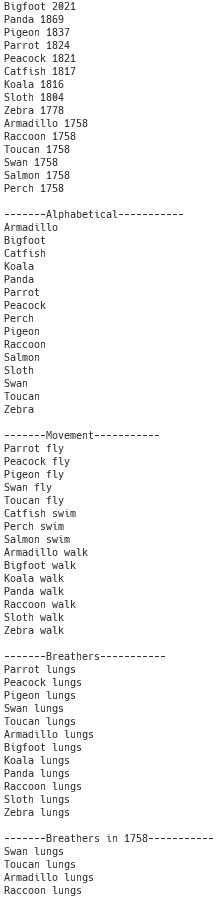
\includegraphics[width = 0.58\columnwidth, center]{lab.png}
  \end{figure}

  \newpage
  \section*{Resultados}
  \subsection*{Problema 1}
  Existen otros lenguajes de programación orientados objetos tales como:

  \begin{enumerate}[label=\alph*.]
    \item KOTLIN (JetBrains /2016)
    \item DART (Google / 2011)
    \item Groovy (JCP /2003)
    \item C$\#$ (Microsoft / 2000)
    \item Python (Rossum / 1991)
  \end{enumerate}
  
  Escoja un lenguaje de programación de la lista y estudie como se presenta el polimorfismo (estático y dinámico).

  \subsection*{Problema 2}
  Traduzca el código del Reino Animal visto en clase al lenguaje seleccionado en el punto anterior y conteste las siguientes preguntas en conclusiones:

  \begin{enumerate}[label=\alph*.]
    \item ¿Qué tan transparente fue realizar dicha traducción? 
    La traducción del código de Java a Dart fue relativamente transparente en términos de lógica y estructura. La mayor parte de la lógica se mantuvo, pero hubo ajustes necesarios debido a diferencias en sintaxis, tipos de datos y manejo de nulos entre los dos lenguajes. En general, la similitud en la orientación a objetos facilitó la traducción, pero se requirió una adaptación para que el código funcionara en el nuevo entorno.

    Mientras que la traducción del código de Java a Kotlin fue altamente transparente y fluida. Kotlin está diseñado para ser compatible con Java, lo que hace que la mayoría de la lógica y estructura del código se traduzcan de manera directa. Kotlin ofrece una sintaxis más concisa y características adicionales que pueden mejorar la legibilidad y el mantenimiento del código.

    \item ¿El concepto de polimorfismo se aplica de la misma manera?
    El concepto de polimorfismo se aplica de manera similar en Java, Dart y Kotlin, ya que todos son lenguajes orientados a objetos que admiten herencia y anulación de métodos. Sin embargo, cada lenguaje tiene su propia sintaxis y características específicas para lograr el polimorfismo. En Java, se utiliza la palabra clave ``extends'' para la herencia y ``@Override'' para anular métodos. En Dart, se hereda de manera implícita y se pueden anular métodos por defecto. En Kotlin, se utiliza ``override'' para anular métodos y se pueden usar ``clases selladas'' para limitar las subclases. A pesar de las diferencias en la implementación, el concepto subyacente de polimorfismo es una característica común en estos lenguajes orientados a objetos.

    \item ¿Se consideraría Java como el padre de estos lenguajes?
    Java no es el ``padre'' de Kotlin y Dart en el sentido de herencia de lenguajes, pero ha influido en su desarrollo. Kotlin se diseñó como una extensión de Java con interoperabilidad completa, mientras que Dart comparte similitudes en programación orientada a objetos. Estos lenguajes se inspiraron en Java y buscan mejorar sus capacidades en áreas específicas. Java influyó en su evolución, pero no son descendientes directos.
  \end{enumerate}

  \textbf{Dart}

  \textbf{Clase \textit{LifeForm}}
  \begin{lstlisting}
abstract class LifeForm {
  void eat(int quantity);

  int getHunger();

  int getYear();

  String move();
  String breathe();
  String reproduce();
}    
  \end{lstlisting}  

  \textbf{Clase \textit{AbstractAnimal}}
  \begin{lstlisting}
import 'LifeForm.dart';

abstract class AbstractAnimal implements LifeForm {
  static int maxId = 0;
  late int hunger;
  late String name;
  late int id;
  late int year;

  AbstractAnimal(String name, int year, int hunger) {
    this.hunger = hunger;
    this.name = name;
    this.year = year;
    maxId++;
    id = maxId;
  }

  AbstractAnimal.namedYear(String name, int year) : this(name, year, 0);

  void eat(int quantity) {
    hunger -= quantity;
    hunger = hunger < 0 ? 0 : hunger;
  }

  String getName() {
    return name;
  }

  int getHunger() {
    return hunger;
  }

  int getId() {
    return id;
  }

  int getYear() {
    return year;
  }

  String move();
  String breathe();
  String reproduce();
}    
  \end{lstlisting}
  
  \textbf{Clase \textit{Mammal}}
  \begin{lstlisting}
import 'AbstractAnimal.dart';

class Mammal extends AbstractAnimal {
  Mammal(String name, int year) : super.namedYear(name, year);

  @override
  String move() {
    return "walk";
  }

  @override
  String breathe() {
    return "lungs";
  }

  @override
  String reproduce() {
    return "live births";
  }
}    
  \end{lstlisting}

  \textbf{Clase \textit{Bird}}
  \begin{lstlisting}
import 'AbstractAnimal.dart';

class Bird extends AbstractAnimal {
  Bird(String name, int year) : super(name, year, 3);

  @override
  String move() {
    return "fly";
  }

  @override
  String breathe() {
    return "lungs";
  }

  @override
  String reproduce() {
    return "eggs";
  }
}    
  \end{lstlisting}

  \textbf{Clase \textit{Fish}}
  \begin{lstlisting}
import 'AbstractAnimal.dart';

class Fish extends AbstractAnimal {
  Fish(String name, int year) : super.namedYear(name, year);

  @override
  String move() {
    return "swim";
  }

  @override
  String breathe() {
    return "gills";
  }

  @override
  String reproduce() {
    return "eggs";
  }
}    
  \end{lstlisting}

  \textbf{\textit{Main}}
  \begin{lstlisting}
import 'AbstractAnimal.dart';
import 'Bird.dart';
import 'Fish.dart';
import 'Mammal.dart';

void main() {
  List<AbstractAnimal> animals = [];
  animals.add(Mammal("Panda", 1869));
  animals.add(Mammal("Zebra", 1778));
  animals.add(Mammal("Koala", 1816));
  animals.add(Mammal("Sloth", 1804));
  animals.add(Mammal("Armadillo", 1758));
  animals.add(Mammal("Raccoon", 1758));
  animals.add(Mammal("Bigfoot", 2021));

  animals.add(Bird("Pigeon", 1837));
  animals.add(Bird("Peacock", 1821));
  animals.add(Bird("Toucan", 1758));
  animals.add(Bird("Parrot", 1824));
  animals.add(Bird("Swan", 1758));

  animals.add(Fish("Salmon", 1758));
  animals.add(Fish("Catfish", 1817));
  animals.add(Fish("Perch", 1758));

  animals.sort((animal1, animal2) => animal2.getYear() - animal1.getYear());
  animals.forEach((animal) {
    print('${animal.getName()} ${animal.getYear()}');
  });
  print("\n-------Alphabetical-----------");
  animals.sort(
      (animal1, animal2) => animal1.getName().compareTo(animal2.getName()));
  animals.forEach((animal) {
    print('${animal.getName()}');
  });

  print("\n-------Movement-----------");
  animals.sort((animal1, animal2) => animal1.move().compareTo(animal2.move()));
  animals.forEach((animal) {
    print('${animal.getName()} ${animal.move()}');
  });

  print("\n-------Breathers-----------");
  animals.forEach((animal) {
    if (animal.breathe() == "lungs") {
      print('${animal.getName()} ${animal.breathe()}');
    }
  });

  print("\n-------Breathers in 1758-----------");
  animals.forEach((animal) {
    if (animal.breathe() == "lungs" && animal.getYear() == 1758) {
      print('${animal.getName()} ${animal.breathe()}');
    }
  });
}    
  \end{lstlisting}

  \textbf{Kotlin}

  \textbf{Clase \textit{LifeForm}}
  \begin{lstlisting}[language=Kotlin]
interface LifeForm {
  fun eat(quantity: Int)
  fun getHunger(): Int
  fun getYear(): Int
  fun move(): String
  fun breathe(): String
  fun reproduce(): String
}
  \end{lstlisting}

  \textbf{Clase \textit{AbstractAnimal}}
  \begin{lstlisting}[language=Kotlin]
import LifeForm

abstract class AbstractAnimal : LifeForm {
  companion object {
    private var maxId = 0
  }

  private var hunger = 0
  private val name: String
  private val id: Int
  private val year: Int

  constructor(name: String, year: Int, hunger: Int) {
    maxId++
    this.id = maxId
    this.hunger = hunger
    this.year = year
    this.name = name
  }

  constructor(name: String, year: Int) : this(name, year, 0)
  
  override fun eat(quantity: Int) {
    hunger -= quantity
    hunger = if (hunger < 0) 0 else hunger
  }

  override fun getHunger(): Int {
    return hunger
  }

  override fun getYear(): Int {
    return year 
  }

  override fun getName(): String {
    return name
  }
  
  abstract override fun move(): String
  abstract override fun breathe(): String
  abstract override fun reproduce(): String
}    
  \end{lstlisting}

  \textbf{Clase \textit{Mammal}}
  \begin{lstlisting}[language=Kotlin]
import AbstractAnimal

class Mammal(name: String, year: Int) : AbstractAnimal(name, year) {
  override fun move(): String {
    return "walk"
  }

  override fun breathe(): String {
    return "lungs"
  }

  override fun reproduce(): String {
    return "live births"
  }

  override fun getName(): String {
    return super.getName()
  }
}    
  \end{lstlisting}

  \textbf{Clase \textit{Bird}}
  \begin{lstlisting}[language=Kotlin]
import AbstractAnimal

class Bird(name: String, year: Int) : AbstractAnimal(name, year, 3) {
  override fun move(): String {
    return "fly"
  }

  override fun breathe(): String {
    return "lungs"
  }

  override fun reproduce(): String {
    return "eggs"
  }

  override fun getName(): String {
    return super.getName()
  }    
}    
  \end{lstlisting}  

  \textbf{Clase \textit{Fish}}
  \begin{lstlisting}[language=Kotlin]
import AbstractAnimal

class Fish(name: String, year: Int) : AbstractAnimal(name, year) {
  override fun move(): String {
    return "swim"
  }

  override fun breathe(): String {
    return "gills"
  }

  override fun reproduce(): String {
    return "eggs"
  }

  override fun getName(): String {
    return super.getName()
  }
}
  \end{lstlisting}

  \textbf{\textit{Main}}
  \begin{lstlisting}[language=Kotlin]
import Mammal
import Bird
import Fish
import AbstractAnimal
import LifeForm

fun main() {
  val animals: MutableList<AbstractAnimal> = mutableListOf()

  animals.add(Mammal("Panda", 1869))
  animals.add(Mammal("Zebra", 1778))
  animals.add(Mammal("Koala", 1816))
  animals.add(Mammal("Sloth", 1804))
  animals.add(Mammal("Armadillo", 1758))
  animals.add(Mammal("Raccoon", 1758))
  animals.add(Mammal("Bigfoot", 2021))

  animals.add(Bird("Pigeon", 1837))
  animals.add(Bird("Peacock", 1821))
  animals.add(Bird("Toucan", 1758))
  animals.add(Bird("Parrot", 1824))
  animals.add(Bird("Swan", 1758))

  animals.add(Fish("Salmon", 1758))
  animals.add(Fish("Catfish", 1817))
  animals.add(Fish("Perch", 1758))

  animals.sortByDescending { it.getYear() }
  animals.forEach { animal ->
    println("${animal.getName()} ${animal.getYear()}")
  }

  println("-------Alphabetical-----------")
  animals.sortBy { it.getName() }
  animals.forEach { animal ->
    println(animal.getName())
  }

  println("-------Movement-----------")
  animals.sortBy { it.move() }
  animals.forEach { animal ->
    println("${animal.getName()} ${animal.move()}")
  }

  println("-------Breathers-----------")
  animals.filter { it.breathe() == "lungs" }.forEach { animal ->
    println("${animal.getName()} ${animal.breathe()}")
  }

  println("-------Breathers in 1758-----------")
  animals.filter { it.breathe() == "lungs" && it.getYear() == 1758 }.forEach { animal ->
    println("${animal.getName()} ${animal.breathe()}")
  }
}    
  \end{lstlisting}

  \subsection*{Problema 3}
  Realice una tabla comparativa de desventajas y ventajas de la sobreescritura y sobrecarga de métodos y concluya desde su punto de vista cuál de las dos maneras de polimorfismo es más útil y porqué.
  
  \newpage
  \textbf{Sobreescritura}
  \begin{table}[h!]
    \footnotesize	
    \begin{tabular}{|p{0.45\columnwidth}|p{0.45\columnwidth}|}
      \hline
      \textbf{Ventajas} & \textbf{Desventajas} \\ \hline
      La capacidad de sobrescribir habilita el polimorfismo, lo que implica que es posible invocar tanto el método de la superclase como el de la subclase de forma consistente, simplificando así la creación de código genérico. & La sobreescritura se encuentra ligada a la herencia, lo que puede dar lugar a una estrecha interconexión entre las clases, lo cual no siempre es la elección ideal en el diseño de software. \\ \hline
      
      Simplifica la tarea de mantener el código, puesto que posibilita la modificación de la forma en que se ejecuta un método en una clase hija sin que ello tenga repercusiones en las demás secciones del código que hacen uso de la clase base. & Se necesita mantener las firmas de los métodos idénticas, lo que implica que no tienes la libertad de alterar la cantidad o tipo de parámetros, ni el tipo de valor de retorno. \\ \hline
      
      La capacidad de sobreescritura permite que las subclases sustituyan la funcionalidad heredada de la superclase, lo que resulta esencial para adaptar el comportamiento de las clases según las necesidades específicas. & \\ \hline
    \end{tabular}
  \end{table}

  \textbf{Sobrecarga}
  \begin{table}[h!]
    \footnotesize	
    \begin{tabular}{|p{0.45\columnwidth}|p{0.45\columnwidth}|}
      \hline
      \textbf{Ventajas} & \textbf{Desventajas} \\ \hline
      Habilita la creación de métodos que comparten el mismo nombre, pero poseen diferentes conjuntos de parámetros, lo que simplifica la creación de métodos con funcionalidades afines. & En situaciones particulares, la sobrecarga puede generar confusión si los argumentos no son lo bastante diferentes entre sí, lo que podría dar lugar a errores de compilación. \\ \hline

      Los nombres de los métodos sobrecargados pueden ser formulados de manera más intuitiva y descriptiva por sí mismos, lo que hace que el código sea más comprensible y fácil de emplear. & El exceso de sobrecarga puede dar lugar a un código enredado y de complicada comprensión, especialmente cuando las diferencias entre las versiones sobrecargadas no son evidentes. \\ \hline


      No se encuentra restringido por las mismas firmas de método que en la sobreescritura, lo que brinda una mayor libertad y flexibilidad en la definición de los métodos. & \\ \hline
    \end{tabular}
  \end{table}

  La decisión entre utilizar la sobreescritura o la sobrecarga se basa en los requisitos de tu programa y la organización de tus clases. Ambos tipos de polimorfismo tienen su utilidad y se aplican en contextos diversos. En general, la sobreescritura es más útil cuando se trabaja con clases relacionadas entre sí, mientras que la sobrecarga es más útil cuando se trabaja con clases que no están relacionadas entre sí.

  \subsection*{Problema 4}
  Implemente la solución del siguiente problema: \url{https://edabit.com/challenge/6RStzK9uub9vHDt53}

  Pero considere la programación de los métodos polimórficos:

  \begin{enumerate}[label=\alph*.]
    \item \textit{sortByLength()} ascendente y descendente
    \item \textit{sortByAlphabet()} de a-z y z-a
  \end{enumerate}

  \textbf{Solución}
  \begin{lstlisting}[language=Java]
import java.util.ArrayList;

public class Problema4{
  public class Sort{
    private static ArrayList<String> split(String s) {
      String[] words = s.split(" ");
      ArrayList<String> wordsAL = new ArrayList<>();
      for (int i = 0; i < words.length; i++)
        wordsAL.add(words[i]);
      return wordsAL;
    }

    private static String append(ArrayList<String> words){
        String result = "";
        for (int i = 0; i < words.size(); i++)
          result += words.get(i) + " ";
        return result;
    }

    public static String sortByLength(String s){
        ArrayList<String> words = new ArrayList<>();
        words = split(s);
        words.sort((word1, word2) -> word1.length() - word2.length());
        return append(words);
    }

    public static String sortByLength(String s, String a){
        ArrayList<String> words = new ArrayList<>();
        words = split(s);
        words.sort((word1, word2) -> word2.length() - word1.length());
        return append(words);
    }

    public static String sortByAlphabet(String s){
        ArrayList<String> words = new ArrayList<>();
        words = split(s);
        words.sort((word1, word2) -> word1.toLowerCase().charAt(0) 
            - word2.toLowerCase().charAt(0));
        return append(words);
    }

    public static String sortByAlphabet(String s, String a){
        ArrayList<String> words = new ArrayList<>();
        words = split(s);
        words.sort((word1, word2) -> word2.toLowerCase().charAt(0) 
            - word1.toLowerCase().charAt(0));
        return append(words);
    }
  }

  public static void main(String[] args) {
    String s = "Hello World in Java";

    System.out.println("String: " + s);
    
    System.out.println("\n- Ordenacion por longitud -");
    System.out.println("Ascendente: " + Sort.sortByLength(s));
    System.out.println("Descendente: " + Sort.sortByLength(s, "s"));
    
    System.out.println("\n- Ordenacion alfabetica -");
    System.out.println("a-z: " + Sort.sortByAlphabet(s));
    System.out.println("z-a: " + Sort.sortByAlphabet(s, "s"));
  }
}    
  \end{lstlisting}

  \textbf{Ejecución}
  \begin{figure}[h!]
    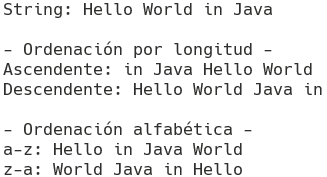
\includegraphics[width=0.6\columnwidth, center]{P4.png}
  \end{figure}

  \section*{Conclusiones}
  El polimorfismo es un concepto fundamental en la programación orientada a objetos que permite que objetos de diferentes tipos puedan interactuar de manera uniforme y eficiente. A lo largo de la información proporcionada, hemos explorado en profundidad el polimorfismo, sus tipos (dinámico y estático) y su aplicación en diferentes contextos
  
  El polimorfismo proporciona flexibilidad y extensibilidad al código, lo que es esencial para el diseño de sistemas de software versátiles y adaptables.

  Entender y aplicar de manera efectiva el polimorfismo es esencial para nosotros los programadores ya que contribuye a la construcción de software de alta calidad.


  \section*{Referencias}
  \small
  Solano, J. (2017, 20 enero). \textit{Manual de prácticas de Programación Orientada a Objetos}. Laboratorio de Computación Salas A y B. \url{http://lcp02.fi-b.unam.mx/} \\

  Zoark. \textit{Sort by Length}. Edabit. \url{https://edabit.com/challenge/6RStzK9uub9vHDt53}
\end{document}